\documentclass[11pt]{article}

\usepackage[dvips]{graphicx}
\usepackage{rotating}

\usepackage{freerbmt09}
\usepackage[utf8x]{inputenc}
\usepackage{times}
\usepackage{natbib}
\usepackage{url}
\usepackage{latexsym}

\title{Implementing an efficient and scalable RBMT service}

\author{Pasquale Minervini\\
  Department of Computer Science \\
  Nonesuch State University \\
  Utopia, NS 12345 \\
  {\tt jane.doe@cs.nsu.edu} \And
  John Smith \\
  Department of Linguistics \\
  Another State University \\
  Collegetown, AS 98765 \\  
  {\tt jsmith@ling.asu.edu}}

\date{}

\begin{document}

\maketitle

\begin{abstract}
Service Oriented Architecture (SOA) is a paradigm for organizing and utilizing distributed services that may be under the 
control of different ownership domains and implemented using various technology stacks. In some contexts, an organization
using an IT infrastructure implementing the SOA paradigm can take a great benefit from an efficient Rule-Based Machine 
Translation (RBMT) service. This paper describes the architecture used to develop an efficient, scalable and easy to integrate
in new and existing business processes RBMT service.
\end{abstract}

\section{Introduction}

Service Oriented Architecture is an architectural paradigm providing  a set of principles of governing concepts used during phases 
of systems development and integration. In such an architecture functionalities are packaged as interoperable services that may be 
used to build infrastructures enabling those with needs (consumers) and those with capabilities (providers) to interact across 
different domains of technology and ownership.

Several new trends in the computer industry rely upon SOA as the enabling foundation, including the automation of Business Process 
Management (BPM) and the multitude of new architecture and design patterns generally referred to as Web 2.0~\cite{web20}.\\

In some contexts, an organization could take a great benefit by integrating a MT service in its IT infrastructure to overcome 
language barriers; for example, a common problem arising when building a Knowledge Base starting from a corpus of free text for
a certain domain (like biomedical, financial etc.) is that the text isn't always in a language that can be comprehended by the
domain experts and/or the knowledge extraction tools beign used. A possible solution to this problem consists in using a Machine
Translation service (eventually using domain-specific dictionaries, rules etc.) to translate the free text from a language to
another with an high accuracy, so that it's then possible to start extracting knowledge from it.\\

\begin{figure}[!ht]
\begin{center}
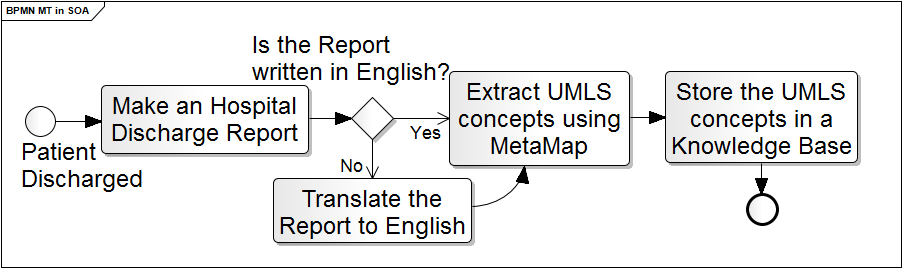
\includegraphics[width=7.5cm]{mtsoa}
\end{center}
\caption{Business Process Model}
\label{fig:mtsoa}
\end{figure}

\section{Service's Interface}


\section{Service's Internals}

\begin{figure}[!ht]
\begin{center}
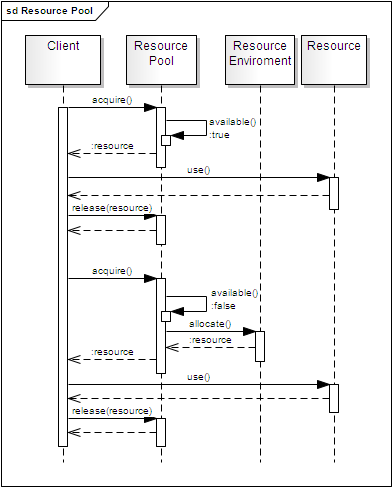
\includegraphics[width=7.5cm]{resource_pool}
\end{center}
\caption{Object Pool}
\label{fig:rp}
\end{figure}

\section{Acknowledgements}



\bibliographystyle{apalike}
\bibliography{freerbmt09}

\end{document}
